\section{两将军问题}

\begin{table}[htbp]
\centering
\begin{tabular}{@{}lll@{}}
\toprule
army 1 \textbackslash{} army 2 & does not attack & attacks \\
\midrule
does not attack & nothing happens & army 2 defeated \\
attacks & army 1 defeated & city captured \\
\bottomrule
\end{tabular}
\end{table}

两将军问题期望：当且仅当军队2发动攻击时，军队1发动攻击。

两将军问题是分布式计算领域中关于“共识一致性”的经典思想实验（1975），它主要探讨的是信道不可靠的问题。

将军们如何决策？
\begin{enumerate}
\item 将军1总是攻击，即使没有收到回应？派送大量信使以增加送达概率。如果全部被俘，2号将军不知道这次攻击，所以1号将军失败。
\item 1号将军只有在收到2号将军的积极回应时才会攻击。
\end{enumerate}

\begin{verbatim}
general 1   general 2
army 1   messengers   army 2
\end{verbatim}

现在1号将军安全。只有2号将军的回应通过并交付至1号，1号才会发动攻击。2号处境同1号。

两将军问题理论上无解（在异步网络中无法达成绝对一致）。

拓展至拜占庭将军问题，由 Lamport 在1982年提出，多将问题升级到了节点不可靠（存在叛徒）的情况。

拓展至拜占庭将军问题 [疑似: 图片内容: general 1 said retreat!]

\begin{figure}[htbp]
\centering
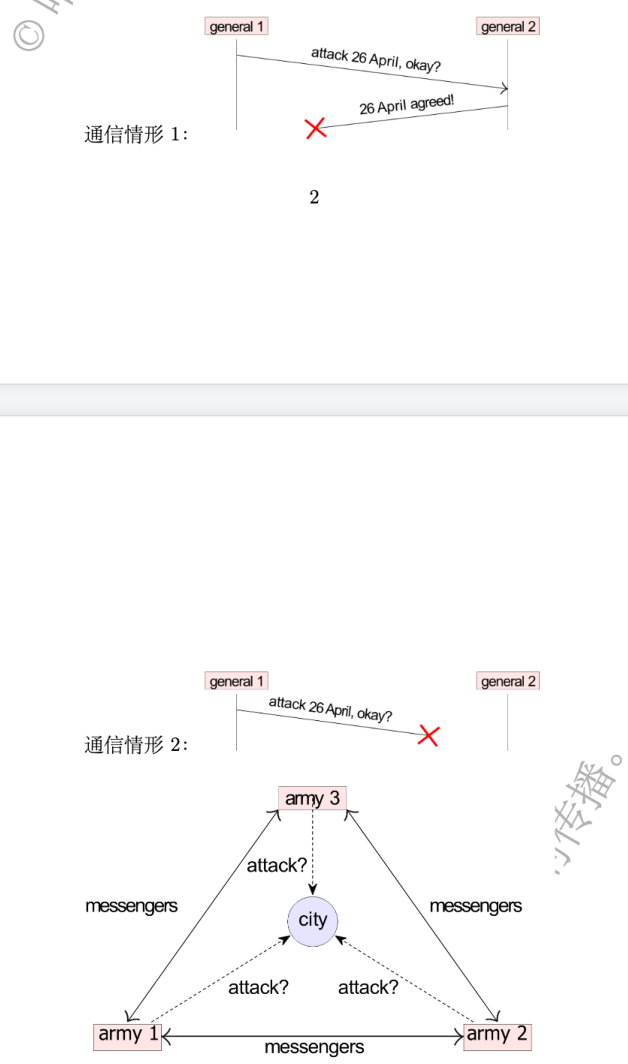
\includegraphics[width=0.8\textwidth]{figures/ch7/ch7_byzantine_generals.png}
\caption{拜占庭将军问题示意}
\end{figure}

\section{拜占庭将军问题的理论解}

假设：一共有 $n$ 位将军，其中包含诚实的将军与恶意的将军，多达 $f$ 名将军可能会有恶意行为；诚实的将军不知道谁是恶意的；恶意的将军们可能会串通密谋；尽管如此，诚实将军们务必达成一致计划。

结论：在消息能可靠传达的前提下，只要叛徒的数量满足 $n > 3f$（即诚实将军超过三分之二），共识就可以达成。（充要条件）

\section{分布式系统模型}

对系统模型进行假设，由以下三部分组成。

\subsection{网络模型}

假设两个节点之间进行双向点对点通信：
\begin{itemize}
\item 可靠链接：有发出就会被收到，但消息可能会被重新排序。
\item 公平-损失链接：是一种对“不完美网络信道”的抽象描述。会丢失、重复或重新排序，不断尝试终会收到。
\item 任意链接（活跃敌手）：恶意对手会干扰消息（窃听、修改、丢弃、欺骗、重放）。
\item 网络分区：在一个分布式系统中，由于网络故障，导致系统被分割成两个或多个互不通信的孤岛（子网）的现象。
\end{itemize}

\begin{quote}
Leslie Lamport, Robert Shostak, and Marshall Pease. 1982. The Byzantine Generals Problem. ACM Trans. Program. Lang. Syst. 4, 3 (July 1982), 382-401. \url{https://doi.org/10.1145/357172.357176}
\end{quote}

\subsection{节点模型}

节点有以下假设情况：
\begin{itemize}
\item 故障-停止：将永远停止执行。节点停止后，其他节点可以检测到其已停止。
\item 故障-恢复：丢失其在内存中的状态，可能会在稍后恢复执行。
\item 故障-省略 (Omission)：无法响应传入请求。
\item 故障-回复 (Response)：无法给出正确的响应。
\item 拜占庭节点，故障-随意 (fail-arbitrary)：故障节点可以[疑似: 做]任何事情，包括崩溃或恶意行为。
\end{itemize}

\subsection{同步模型}

同步假设如下：
\begin{itemize}
\item 同步：消息延迟不大于已知上限；节点以已知速度执行算法。
\item 部分同步：大部分时间是同步的，但在某些不可预知时刻，系统会进入异步。
\item 异步：[疑似: HERBIE. WARN BARRE.]
\end{itemize}

\section{3 CAP 定理}

\textbf{一致性 (C)}：系统中的所有节点都同意系统当前状态。

\textbf{可用性 (A)}：系统提供的服务必须一直处于可用状态，对于用户的每一个操作请求总是能够在有限时间内返回结果。

\textbf{分区容错性 (P)}：分布式系统在遇到任何网络分区故障（即节点间无法通信）时，仍能对外提供满足一致性或可用性的服务。

CAP 定理：在一个分布式系统中，一致性 (Consistency)、可用性 (Availability)、分区容错性 (Partition tolerance)，这三个要素最多只能同时实现两点，不可能三者兼顾。

\begin{figure}[htbp]
\centering
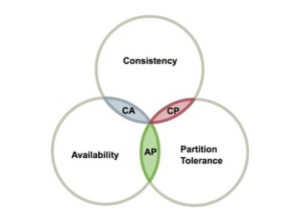
\includegraphics[width=0.8\textwidth]{figures/ch7/ch7_cap_theorem.png}
\caption{CAP 定理三者关系}
\end{figure}

\section{故障检测}

\begin{itemize}
\item 故障检测器：检测另一节点是否有故障的算法。
\item 发送消息，等待响应，若超时 [疑似: BAAR. MILAM.]。
\item 无法区分：崩溃节点、暂时无响应节点、丢失消息和延迟消息。
\end{itemize}

\begin{verbatim}
Periodic ping (Cr)  ack (Ca)
Periodic Cr) => Ca)
具体实现方法：每隔 T 给 p 发送 ping，等待 (T + Ac) 超时，若超时则疑似挂了。
同步情形：Δs = max network delay - min network delay
异步情形：Δs = k (observed delay); k > 1
\end{verbatim}

故障检测基于超时的完美故障检测器，仅存在于具有可靠链路、同步的崩溃-停止系统中。

最终完美故障检测器：
\begin{itemize}
\item 可能将节点临时标记为崩溃，即使它正确运行。
\item 可能将节点临时标记为正常的，即使它已经崩溃。
\item 但最终，将节点标记为已崩溃当且仅当它已崩溃。
\end{itemize}

实际情况：检测不会是即时的，可能会有虚假超时。

\section{故障模型}

\section{广播协议}

广播（多播）为组通信：
\begin{itemize}
\item 向所有节点发送消息，所有节点传递消息。（组成员集合可以是固定的（静态的）也可以是动态的。）
\item 如果一个节点出现故障，则其余组成员继续工作。
\end{itemize}

系统建模：
\begin{itemize}
\item 尽力交付：最大努力（可能会丢弃消息）。
\item 异步/部分同步时序模型：消息延迟没有上限。
\end{itemize}

\subsection{常见多播/广播顺序对比}

\begin{table}[htbp]
\centering
\begin{tabular}{@{}llll@{}}
\toprule
顺序类型 & 约束范围 & 典型场景 & 开销 \\
\midrule
FIFO 序广播 & 仅保证同一发送者的消息按发送顺序交付；不同发送者的消息无顺序保证 & 单源数据流、日志复制 & 最低 \\
因果序广播 & 保证所有存在因果依赖 (happens-before) 关系的消息按因果顺序交付；并发消息无强制顺序 & 协同编辑、聊天 & 中等（向量时钟） \\
全序广播 & 所有进程看到的全局交付顺序完全一致 & 分布式锁、多副本一致性 & 高（协调/共识协议） \\
FIFO-全序广播 & 同一发送者 FIFO 顺序基础上增加全局顺序约束；所有进程至全局交付顺序一致 & 分布式数据库、金融系统 & 高（共识算法与序列号校验） \\
\bottomrule
\end{tabular}
\end{table}

\subsection{广播协议演示}

\subsection{广播的现实问题}

\begin{itemize}
\item 网络异步性与延迟不确定性
\item 消息爆炸与带宽瓶颈
\item 消息乱序与重放 (Ordering \& Replay)
\item 节点成员变更的动态性
\item 拜占庭故障与安全性 (Byzantine Faults)
\end{itemize}

\section{FLP 不可能性}

分布式系统的一个根本问题是，如何在存在故障的情况下实现系统的整体可靠性。这通常需要协调各个进程以达成共识，即：就运行过程中所需的某些数据达成一致。

% image
% \includegraphics[width=0.8\textwidth]{../work/figures/placeholder}
% 请将 placeholder 替换为实际图片名称

在 FIFO 序基础上增加全局顺序约束：所有进程全局交付顺序一致，常见于分布式数据库、金融系统，开销高（共识算法与序列号校验）。
